\documentclass[12pt,]{article}
\usepackage{lmodern}
\usepackage{amssymb,amsmath}
\usepackage{ifxetex,ifluatex}
\usepackage{fixltx2e} % provides \textsubscript
\ifnum 0\ifxetex 1\fi\ifluatex 1\fi=0 % if pdftex
  \usepackage[T1]{fontenc}
  \usepackage[utf8]{inputenc}
\else % if luatex or xelatex
  \ifxetex
    \usepackage{mathspec}
  \else
    \usepackage{fontspec}
  \fi
  \defaultfontfeatures{Ligatures=TeX,Scale=MatchLowercase}
    \setmainfont[]{Times New Roman}
\fi
% use upquote if available, for straight quotes in verbatim environments
\IfFileExists{upquote.sty}{\usepackage{upquote}}{}
% use microtype if available
\IfFileExists{microtype.sty}{%
\usepackage{microtype}
\UseMicrotypeSet[protrusion]{basicmath} % disable protrusion for tt fonts
}{}
\usepackage[margin=2cm]{geometry}
\usepackage{hyperref}
\hypersetup{unicode=true,
            pdftitle={UV Absorbance characteristics in Northern Lakes},
            pdfauthor={Rachel Bash},
            pdfborder={0 0 0},
            breaklinks=true}
\urlstyle{same}  % don't use monospace font for urls
\usepackage{color}
\usepackage{fancyvrb}
\newcommand{\VerbBar}{|}
\newcommand{\VERB}{\Verb[commandchars=\\\{\}]}
\DefineVerbatimEnvironment{Highlighting}{Verbatim}{commandchars=\\\{\}}
% Add ',fontsize=\small' for more characters per line
\usepackage{framed}
\definecolor{shadecolor}{RGB}{248,248,248}
\newenvironment{Shaded}{\begin{snugshade}}{\end{snugshade}}
\newcommand{\KeywordTok}[1]{\textcolor[rgb]{0.13,0.29,0.53}{\textbf{#1}}}
\newcommand{\DataTypeTok}[1]{\textcolor[rgb]{0.13,0.29,0.53}{#1}}
\newcommand{\DecValTok}[1]{\textcolor[rgb]{0.00,0.00,0.81}{#1}}
\newcommand{\BaseNTok}[1]{\textcolor[rgb]{0.00,0.00,0.81}{#1}}
\newcommand{\FloatTok}[1]{\textcolor[rgb]{0.00,0.00,0.81}{#1}}
\newcommand{\ConstantTok}[1]{\textcolor[rgb]{0.00,0.00,0.00}{#1}}
\newcommand{\CharTok}[1]{\textcolor[rgb]{0.31,0.60,0.02}{#1}}
\newcommand{\SpecialCharTok}[1]{\textcolor[rgb]{0.00,0.00,0.00}{#1}}
\newcommand{\StringTok}[1]{\textcolor[rgb]{0.31,0.60,0.02}{#1}}
\newcommand{\VerbatimStringTok}[1]{\textcolor[rgb]{0.31,0.60,0.02}{#1}}
\newcommand{\SpecialStringTok}[1]{\textcolor[rgb]{0.31,0.60,0.02}{#1}}
\newcommand{\ImportTok}[1]{#1}
\newcommand{\CommentTok}[1]{\textcolor[rgb]{0.56,0.35,0.01}{\textit{#1}}}
\newcommand{\DocumentationTok}[1]{\textcolor[rgb]{0.56,0.35,0.01}{\textbf{\textit{#1}}}}
\newcommand{\AnnotationTok}[1]{\textcolor[rgb]{0.56,0.35,0.01}{\textbf{\textit{#1}}}}
\newcommand{\CommentVarTok}[1]{\textcolor[rgb]{0.56,0.35,0.01}{\textbf{\textit{#1}}}}
\newcommand{\OtherTok}[1]{\textcolor[rgb]{0.56,0.35,0.01}{#1}}
\newcommand{\FunctionTok}[1]{\textcolor[rgb]{0.00,0.00,0.00}{#1}}
\newcommand{\VariableTok}[1]{\textcolor[rgb]{0.00,0.00,0.00}{#1}}
\newcommand{\ControlFlowTok}[1]{\textcolor[rgb]{0.13,0.29,0.53}{\textbf{#1}}}
\newcommand{\OperatorTok}[1]{\textcolor[rgb]{0.81,0.36,0.00}{\textbf{#1}}}
\newcommand{\BuiltInTok}[1]{#1}
\newcommand{\ExtensionTok}[1]{#1}
\newcommand{\PreprocessorTok}[1]{\textcolor[rgb]{0.56,0.35,0.01}{\textit{#1}}}
\newcommand{\AttributeTok}[1]{\textcolor[rgb]{0.77,0.63,0.00}{#1}}
\newcommand{\RegionMarkerTok}[1]{#1}
\newcommand{\InformationTok}[1]{\textcolor[rgb]{0.56,0.35,0.01}{\textbf{\textit{#1}}}}
\newcommand{\WarningTok}[1]{\textcolor[rgb]{0.56,0.35,0.01}{\textbf{\textit{#1}}}}
\newcommand{\AlertTok}[1]{\textcolor[rgb]{0.94,0.16,0.16}{#1}}
\newcommand{\ErrorTok}[1]{\textcolor[rgb]{0.64,0.00,0.00}{\textbf{#1}}}
\newcommand{\NormalTok}[1]{#1}
\usepackage{longtable,booktabs}
\usepackage{graphicx,grffile}
\makeatletter
\def\maxwidth{\ifdim\Gin@nat@width>\linewidth\linewidth\else\Gin@nat@width\fi}
\def\maxheight{\ifdim\Gin@nat@height>\textheight\textheight\else\Gin@nat@height\fi}
\makeatother
% Scale images if necessary, so that they will not overflow the page
% margins by default, and it is still possible to overwrite the defaults
% using explicit options in \includegraphics[width, height, ...]{}
\setkeys{Gin}{width=\maxwidth,height=\maxheight,keepaspectratio}
\IfFileExists{parskip.sty}{%
\usepackage{parskip}
}{% else
\setlength{\parindent}{0pt}
\setlength{\parskip}{6pt plus 2pt minus 1pt}
}
\setlength{\emergencystretch}{3em}  % prevent overfull lines
\providecommand{\tightlist}{%
  \setlength{\itemsep}{0pt}\setlength{\parskip}{0pt}}
\setcounter{secnumdepth}{5}
% Redefines (sub)paragraphs to behave more like sections
\ifx\paragraph\undefined\else
\let\oldparagraph\paragraph
\renewcommand{\paragraph}[1]{\oldparagraph{#1}\mbox{}}
\fi
\ifx\subparagraph\undefined\else
\let\oldsubparagraph\subparagraph
\renewcommand{\subparagraph}[1]{\oldsubparagraph{#1}\mbox{}}
\fi

%%% Use protect on footnotes to avoid problems with footnotes in titles
\let\rmarkdownfootnote\footnote%
\def\footnote{\protect\rmarkdownfootnote}

%%% Change title format to be more compact
\usepackage{titling}

% Create subtitle command for use in maketitle
\providecommand{\subtitle}[1]{
  \posttitle{
    \begin{center}\large#1\end{center}
    }
}

\setlength{\droptitle}{-2em}

  \title{UV Absorbance characteristics in Northern Lakes}
    \pretitle{\vspace{\droptitle}\centering\huge}
  \posttitle{\par}
  \subtitle{\url{https://github.com/rachelbash/absorbance-data-project}}
  \author{Rachel Bash}
    \preauthor{\centering\large\emph}
  \postauthor{\par}
      \predate{\centering\large\emph}
  \postdate{\par}
    \date{April 16th, 2019}


\begin{document}
\maketitle
\begin{abstract}
Absorbance values were measured during a portion of the Cascade Project
in the Northern Temperate Lakes LTER network for lakes in northern
Wisconsin and the southern part of Michigan's Upper Peninsula.
Absorption of light in lakes can be an important variable to study in
long-term monitoring programs because of its high correlations between
other physical characterstics of lakes, such as dissolved organic carbon
content. This study examined the variables that contributed to overall
absorbance values and found that depth, dissolved organic carbon, total
particulate carbon, and lake were significant predictors that informed
the linear model. The study also examined absorbance changes over time
in five lakes. East Long Lake and West Long Lake had decreasing
absorbance values over time, while Tuesday and Peter Lakes had
increasing absorbance values over time. Paul Lake did not display any
significant trend over time.
\end{abstract}

\newpage

\tableofcontents  \newpage
\listoftables
1 Data Summary
\ldots{}\ldots{}\ldots{}\ldots{}\ldots{}\ldots{}\ldots{}\ldots{}\ldots{}\ldots{}\ldots{}\ldots{}\ldots{}\ldots{}\ldots{}\ldots{}\ldots{}\ldots{}\ldots{}\ldots{}\ldots{}\ldots{}\ldots{}\ldots{}.6
\newpage
\listoffigures  \newpage

\section{Research Question and
Rationale}\label{research-question-and-rationale}

Absorbance is a unit-less measurement that describes how much a
substance can absorb light over a certain range of wavelength. The
absorbance values of water samples from lakes can provide details
regarding its physical characteristics and the health of the lake. The
amount of light entering a lake is a component that drives
photosynthesis and lake metabolism (Thrane, 2014). Additionally, lake
temperature and its absorbance characteristics are deeply intertwined.
With the right equipment, absorbance is fairly easy to measure.
Therefore, measuring absorbance in lakes can give researchers insight
into other processes happening that depend in part on sunlight, such as
algal growth or temperature-dependent biological activities.

This research project intends to answer three main questions:

\begin{itemize}
\tightlist
\item
  What contributes to absorbance values in five lakes located in
  Michigan's Upper Peninsula?
\item
  Are absorbance values between lakes different?
\item
  Do absorbance values in these five study lakes change over time?
\end{itemize}

The data that answer these questions come from the North Temperate Lakes
Project, which seeks to measure data on carbon and other related
variables in lakes. My analysis of the data provides a model that shows
the variables that best predict absorbance values and also takes a
closer look at how absorbance values have changed over time in different
lakes. Time variations in absorbance have implications that other
physical characteristics are changing, which may damage biota in the
lakes or bring about significant changes in the greater ecosystem that
surrounds the lake. Because absorbance value changes can be an
indicator, it is important to study this measurement and what
contributes to the changes.

\newpage

\section{Dataset Information}\label{dataset-information}

The dataset was collected from 1984 to 2016 by researchers working for
the Cascade Project and Northern Temperate Lakes Long-Term Ecological
Research Network (NTL-LTER) at a total of 14 sites. Samples of water
were collected, and then were measured. Measurements included dissolved
organic and inorganic carbon, particulate organic matter, partial
pressure of carbon dioxide, and absorbance. Absorbance was measured
using a spectrophotometer at a wavelength of 440nanometers.

For some variables, a water depth sample was taken that was measured in
meters, while in others, samples were taken to reflect a depth that was
proportional across all lakes. Therefore, Hypolimnion, Epilimnion,
Metalimnion, and pooled mixed layer (PML) are also included as depth
values. All water samples were taken with a syringe and then filtered
through a mesh filter in order to remove any large debris or
zooplankton.

\begin{longtable}[]{@{}ll@{}}
\toprule
\begin{minipage}[b]{0.26\columnwidth}\raggedright\strut
Data Summary\strut
\end{minipage} & \begin{minipage}[b]{0.30\columnwidth}\raggedright\strut
Relevant Information\strut
\end{minipage}\tabularnewline
\midrule
\endhead
\begin{minipage}[t]{0.26\columnwidth}\raggedright\strut
Date range\strut
\end{minipage} & \begin{minipage}[t]{0.30\columnwidth}\raggedright\strut
1984-06-03 to 2016-08-17\strut
\end{minipage}\tabularnewline
\begin{minipage}[t]{0.26\columnwidth}\raggedright\strut
Retrieved from\strut
\end{minipage} & \begin{minipage}[t]{0.30\columnwidth}\raggedright\strut
NTL - LTER Cascade Project at North Temperate Lakes LTER Core Data
Carbon\strut
\end{minipage}\tabularnewline
\begin{minipage}[t]{0.26\columnwidth}\raggedright\strut
Structure\strut
\end{minipage} & \begin{minipage}[t]{0.30\columnwidth}\raggedright\strut
15 variables with 13,557 observations\strut
\end{minipage}\tabularnewline
\begin{minipage}[t]{0.26\columnwidth}\raggedright\strut
Column variables\strut
\end{minipage} & \begin{minipage}[t]{0.30\columnwidth}\raggedright\strut
Lake ID, Lake Name, Year, Day No., Date, Depth, Depth ID, TPC, TPN, DIC,
PCO2 air, PCO2 water, DOC, Absorbance\strut
\end{minipage}\tabularnewline
\begin{minipage}[t]{0.26\columnwidth}\raggedright\strut
Lakes sampled\strut
\end{minipage} & \begin{minipage}[t]{0.30\columnwidth}\raggedright\strut
Crampton Lake, East Long Lake, Hummingbird Lake, Long Lake, Morris Lake,
North Gate Bog, Paul Lake, Peter Lake, Reddington Lake, Roach Lake,
Tender Bog, Tuesday Lake, Ward Lake, West Long Lake\strut
\end{minipage}\tabularnewline
\bottomrule
\end{longtable}

\newpage

\section{Exploratory Data Analysis and
Wrangling}\label{exploratory-data-analysis-and-wrangling}

\subsection{Importing raw data and identifying its
attributes}\label{importing-raw-data-and-identifying-its-attributes}

\begin{Shaded}
\begin{Highlighting}[]
\KeywordTok{colnames}\NormalTok{(carbon.data)}
\end{Highlighting}
\end{Shaded}

\begin{verbatim}
##  [1] "lakeid"     "lakename"   "year4"      "daynum"     "sampledate"
##  [6] "depth"      "depth_id"   "tpc"        "tpn"        "DIC_mg"    
## [11] "DIC_uM"     "air_pco2"   "water_pco2" "doc"        "absorbance"
\end{verbatim}

\begin{Shaded}
\begin{Highlighting}[]
\KeywordTok{str}\NormalTok{(carbon.data)}
\end{Highlighting}
\end{Shaded}

\begin{verbatim}
## 'data.frame':    13557 obs. of  15 variables:
##  $ lakeid    : Factor w/ 14 levels "E","H","L","Long",..: 3 3 3 3 3 8 8 8 8 8 ...
##  $ lakename  : Factor w/ 14 levels "Crampton Lake",..: 7 7 7 7 7 8 8 8 8 8 ...
##  $ year4     : int  1984 1984 1984 1984 1984 1984 1984 1984 1984 1984 ...
##  $ daynum    : int  155 155 155 155 155 156 156 156 156 156 ...
##  $ sampledate: Date, format: "1984-06-03" "1984-06-03" ...
##  $ depth     : Factor w/ 231 levels "0","0.1","0.15",..: 1 62 102 140 180 1 62 102 140 202 ...
##  $ depth_id  : int  1 2 3 4 5 1 2 3 4 5 ...
##  $ tpc       : num  NA NA NA NA NA NA NA NA NA NA ...
##  $ tpn       : num  NA NA NA NA NA NA NA NA NA NA ...
##  $ DIC_mg    : num  1.45 1.82 1.51 1.47 2.69 2.85 2.84 3.27 2.98 7.26 ...
##  $ DIC_uM    : num  121 152 126 122 224 ...
##  $ air_pco2  : num  NA NA NA NA NA NA NA NA NA NA ...
##  $ water_pco2: num  NA NA NA NA NA NA NA NA NA NA ...
##  $ doc       : num  NA NA NA NA NA NA NA NA NA NA ...
##  $ absorbance: num  NA NA NA NA NA NA NA NA NA NA ...
\end{verbatim}

\begin{Shaded}
\begin{Highlighting}[]
\KeywordTok{summary}\NormalTok{(carbon.data)}
\end{Highlighting}
\end{Shaded}

\begin{verbatim}
##      lakeid               lakename        year4          daynum     
##  R      :3887   Peter Lake    :3887   Min.   :1984   Min.   : 82.0  
##  L      :3852   Paul Lake     :3852   1st Qu.:1993   1st Qu.:166.0  
##  T      :1818   Tuesday Lake  :1818   Median :1999   Median :192.0  
##  W      :1571   West Long Lake:1571   Mean   :2000   Mean   :192.4  
##  E      :1435   East Long Lake:1435   3rd Qu.:2007   3rd Qu.:218.0  
##  M      : 456   Crampton Lake : 456   Max.   :2016   Max.   :310.0  
##  (Other): 538   (Other)       : 538                                 
##    sampledate                 depth         depth_id           tpc        
##  Min.   :1984-06-03   0          :1719   Min.   :-2.000   Min.   : 0.100  
##  1st Qu.:1993-06-16   Metalimnion:1297   1st Qu.: 1.000   1st Qu.: 0.580  
##  Median :1999-07-06   Hypolimnion:1020   Median : 3.000   Median : 0.890  
##  Mean   :2000-07-14   PML        : 876   Mean   : 2.775   Mean   : 1.110  
##  3rd Qu.:2007-08-28   Epilimnion : 570   3rd Qu.: 5.000   3rd Qu.: 1.305  
##  Max.   :2016-08-17   (Other)    :7918   Max.   : 7.000   Max.   :11.860  
##                       NA's       : 157   NA's   :170      NA's   :11410   
##       tpn            DIC_mg           DIC_uM            air_pco2    
##  Min.   :0.000   Min.   : 0.023   Min.   :   1.917   Min.   :197.7  
##  1st Qu.:0.070   1st Qu.: 0.812   1st Qu.:  67.625   1st Qu.:343.4  
##  Median :0.103   Median : 1.322   Median : 110.167   Median :362.9  
##  Mean   :0.149   Mean   : 2.310   Mean   : 192.487   Mean   :360.4  
##  3rd Qu.:0.180   3rd Qu.: 1.968   3rd Qu.: 164.000   3rd Qu.:379.0  
##  Max.   :2.170   Max.   :48.599   Max.   :4049.883   Max.   :608.1  
##  NA's   :11409   NA's   :3642     NA's   :3642       NA's   :12411  
##    water_pco2          doc           absorbance   
##  Min.   :   0.0   Min.   : 2.710   Min.   :0.011  
##  1st Qu.: 478.0   1st Qu.: 4.570   1st Qu.:0.060  
##  Median : 838.5   Median : 5.603   Median :0.146  
##  Mean   :1012.3   Mean   : 6.932   Mean   :0.194  
##  3rd Qu.:1175.6   3rd Qu.: 8.370   3rd Qu.:0.265  
##  Max.   :9348.2   Max.   :44.080   Max.   :1.213  
##  NA's   :12411    NA's   :9993     NA's   :10658
\end{verbatim}

\begin{Shaded}
\begin{Highlighting}[]
\KeywordTok{dim}\NormalTok{(carbon.data)}
\end{Highlighting}
\end{Shaded}

\begin{verbatim}
## [1] 13557    15
\end{verbatim}

\begin{Shaded}
\begin{Highlighting}[]
\KeywordTok{summary}\NormalTok{(carbon.data}\OperatorTok{$}\NormalTok{absorbance)}
\end{Highlighting}
\end{Shaded}

\begin{verbatim}
##    Min. 1st Qu.  Median    Mean 3rd Qu.    Max.    NA's 
##   0.011   0.060   0.146   0.194   0.265   1.213   10658
\end{verbatim}

\begin{Shaded}
\begin{Highlighting}[]
\KeywordTok{class}\NormalTok{(carbon.data}\OperatorTok{$}\NormalTok{depth)}
\end{Highlighting}
\end{Shaded}

\begin{verbatim}
## [1] "factor"
\end{verbatim}

\begin{Shaded}
\begin{Highlighting}[]
\KeywordTok{head}\NormalTok{(carbon.data}\OperatorTok{$}\NormalTok{depth, }\DecValTok{10}\NormalTok{)}
\end{Highlighting}
\end{Shaded}

\begin{verbatim}
##  [1] 0   1   2   3.5 5.5 0   1   2   3.5 7  
## 231 Levels: 0 0.1 0.15 0.17 0.18 0.19 0.2 0.21 0.22 0.23 0.25 0.28 ... surface
\end{verbatim}

These exploratory commands above function as helpful tools that help me
see what kind of shape my data are in. It shows me the size of the data
frame, how many NA's I have, what variables I am working with, the
classes of my variables, and basic summary statistics. These are
important to know and help inform me when making decisions about further
analysis. An meaningful detail I discovered while doing the initial
exploratory data analysis is that the depth variable has both numeric
and factor-level observations, which is why its class is listed as
\texttt{factor}. In other words, depth was measured in both numeric
terms (1 meter, 13 meters, etc), but also in thermally stratified terms,
such as Hypolimnion, Metalimnion, and Epilimnion. This was an important
discovery that led to further data wrangling and filtering of this
specific variable.

\subsection{Visualizing the data}\label{visualizing-the-data}

As seen by \autoref{fig:foo}, Absorbance values are not normally
distributed. This is expected, as we are dealing with ecological data.

\begin{figure}
\centering
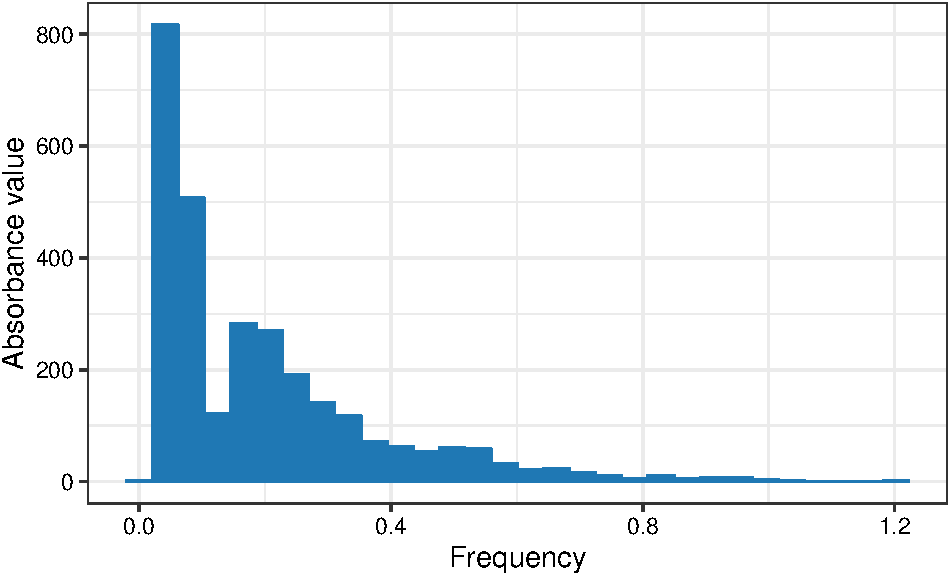
\includegraphics{Bash_ENV872_Project_files/figure-latex/foo-1.pdf}
\caption{\label{fig:foo}Absorbance frequency}
\end{figure}

\begin{figure}
\centering
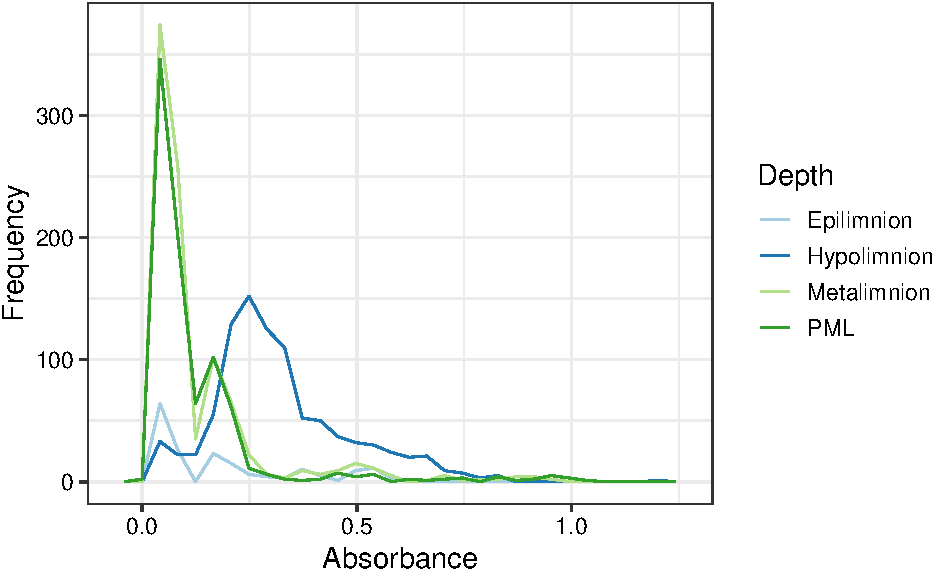
\includegraphics{Bash_ENV872_Project_files/figure-latex/freqpol-1.pdf}
\caption{\label{fig:freqpol}Absorbance frequency by depth category}
\end{figure}

Similarly, \autoref{fig:freqpol} shows that different levels of depth
(factor) had difference absorbance frequency values. It was helpful to
create this graph to show that absorbance was measured at multiple
different water depth levels.

\begin{figure}
\centering
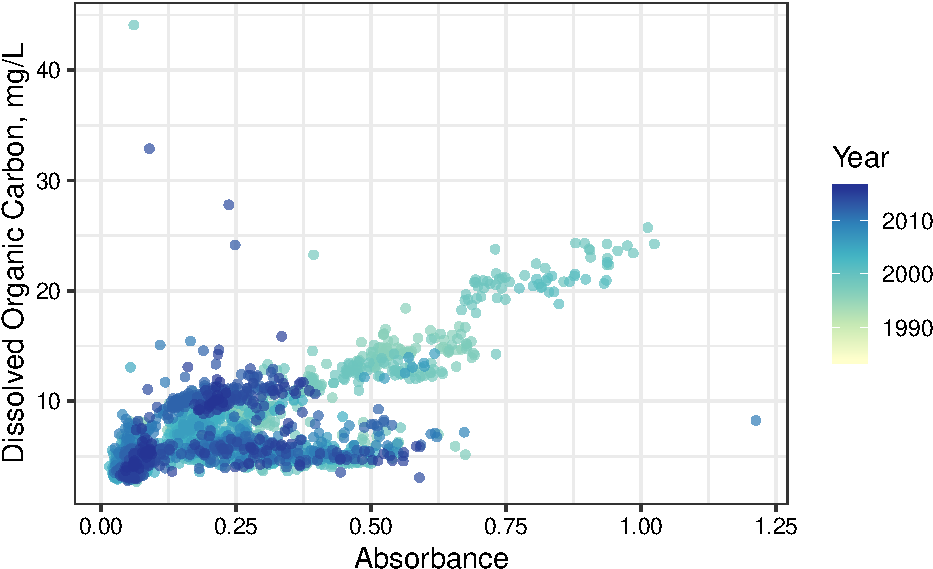
\includegraphics{Bash_ENV872_Project_files/figure-latex/absorbdoc-1.pdf}
\caption{\label{fig:absorbdoc} Disolved organic carbon and absorbance
relationship by year}
\end{figure}

\autoref{fig:absorbdoc} shows a positive relationship between dissolved
organic carbon and absorbance, with a layer of color by year. This
result is expected, and it gave me a good sense of what to expect during
my analysis portion of the project. It is interesting to note that as
time went on, measures for both absorbance and for DOC began to shrink
to smaller values, as seen with the color gradient by year. Another
thing this plot tells me is that absorbance probably wasn't measured in
the early times of data collection, as there are no points before 1990,
as indicated by the yellow color on the graph.

\subsection{Data Wrangling}\label{data-wrangling}

\begin{Shaded}
\begin{Highlighting}[]
\NormalTok{carbon.data.processed <-}\StringTok{ }\NormalTok{carbon.data }\OperatorTok
\StringTok{  }\KeywordTok{filter}\NormalTok{(depth }\OperatorTok\StringTok{ }\KeywordTok{c}\NormalTok{(}\StringTok{"PML"}\NormalTok{, }\StringTok{"Hypolimnion"}\NormalTok{, }\StringTok{"Epilimnion"}\NormalTok{, }\StringTok{"Metalimnion"}\NormalTok{)) }\OperatorTok
\StringTok{  }\KeywordTok{filter}\NormalTok{(lakename }\OperatorTok\StringTok{ }\KeywordTok{c}\NormalTok{(}\StringTok{"Peter Lake"}\NormalTok{, }\StringTok{"Paul Lake"}\NormalTok{, }\StringTok{"East Long Lake"}\NormalTok{, }\StringTok{"Tuesday Lake"}\NormalTok{, }\StringTok{"West Long Lake"}\NormalTok{)) }\OperatorTok
\StringTok{  }\KeywordTok{select}\NormalTok{(lakename}\OperatorTok{:}\NormalTok{depth_id, DIC_mg, doc, absorbance, tpc)}
\end{Highlighting}
\end{Shaded}

There were many things to consider when wrangling my data to a more
manageable and workable dataset. I noticed that all absorbance values
had associated depth measurements using only the thermally stratified
depth categories. Therefore, I filtered out any depth that was measured
in meters, in order to simplify the process. Next, I chose the five
lakes in the dataset that had the most number of data points. Shortening
the lake list from 14 to 5 gives the research project a more focused
view and potentially stronger relationships among variables. Lastly, I
selected only the columns that I wanted to study and that could be
analyzed in relation to absorbance values. These variables included lake
name, depth, dissolved inorganic carbon, dissolved organic carbon, total
particulate carbon, and absorbance.

\subsection{Correlation between continuous
variables}\label{correlation-between-continuous-variables}

\begin{figure}
\centering
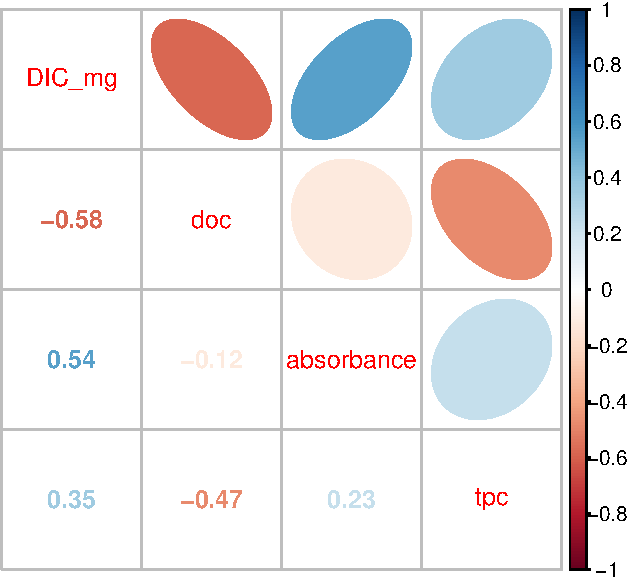
\includegraphics{Bash_ENV872_Project_files/figure-latex/corr-1.pdf}
\caption{\label{fig:corr} Correlation plot between continuous variables}
\end{figure}

The last piece of data exploration I completed was visualizing the
correlation between the continuous variables in the data.
\autoref{fig:corr} illustrates the relationships between each of the
continuous variables in question. All relationship correlations range
pretty low to moderate, with DOC and absorbance having the lowest
correlation coefficient of -0.12, and DIC and DOC having the highest
negative correlation coefficient of -0.58. It is important to consider
this visualization critically, as the data have been thoroughly reduced
at this point, leaving much fewer data points than what we started with,
which could manipulate the strength (or weakness) of these correlation
coefficients.

\newpage

\section{Analysis}\label{analysis}

\subsection{Differences in absorbance values across
lakes}\label{differences-in-absorbance-values-across-lakes}

It was important for me to know whether absorbance values were
significantly different across the five lakes of interest. This can be
answered by a simple ANOVA test. However, the data must meet certain
criteria. Fist, data had to be normally distributed, and second, equal
variance across groups must exist. I tested these assumptions using the
Shapiro Wilk test and the Bartlett test, respectively. Both tests
resulted in significant p-values, indicating that the data fail the
tests for normality and equal variances.

Therefore, another method had to be utilized. I opted for a
non-parametric test called the Kruskal Wallis test, a great alternative
to ANOVAs. Here, I received a significant p-value result, indicating
that there is a significant difference in absorbance values across
different lakes (chi-squared = 739.62, df = 4, p-value \textless{}
2.2e-16). A non-parametric post-hoc test (Dunn Test) reveals that all
lakes' mean absorbances values are significantly different from all
other lakes (p-values \textless{} 0.05). \autoref{fig:vio} illustrates
how absorbance values vary vastly by lake. Even though all of these
lakes are located close to each other in Michigan's Upper Peninsula
along the Wisconsin border, it is clear that absorbance values can vary
greatly among them. Even Peter and Paul Lakes, whose mean absorbance
values do look fairly close, do possess a significant p-value in the
post-hoc test, indicating that they are statistically significantly
different from one another.

\begin{Shaded}
\begin{Highlighting}[]
\CommentTok{# test for normality}
\KeywordTok{shapiro.test}\NormalTok{(carbon.data.processed}\OperatorTok{$}\NormalTok{absorbance}
\NormalTok{             [carbon.data.processed}\OperatorTok{$}\NormalTok{lakename }\OperatorTok{==}\StringTok{ "Tuesday Lake"}\NormalTok{])}
\end{Highlighting}
\end{Shaded}

\begin{verbatim}
## 
##  Shapiro-Wilk normality test
## 
## data:  carbon.data.processed$absorbance[carbon.data.processed$lakename ==     "Tuesday Lake"]
## W = 0.97269, p-value = 8.155e-06
\end{verbatim}

\begin{Shaded}
\begin{Highlighting}[]
\KeywordTok{shapiro.test}\NormalTok{(carbon.data.processed}\OperatorTok{$}\NormalTok{absorbance}
\NormalTok{             [carbon.data.processed}\OperatorTok{$}\NormalTok{lakename }\OperatorTok{==}\StringTok{ "Paul Lake"}\NormalTok{])}
\end{Highlighting}
\end{Shaded}

\begin{verbatim}
## 
##  Shapiro-Wilk normality test
## 
## data:  carbon.data.processed$absorbance[carbon.data.processed$lakename ==     "Paul Lake"]
## W = 0.71627, p-value < 2.2e-16
\end{verbatim}

\begin{Shaded}
\begin{Highlighting}[]
\KeywordTok{shapiro.test}\NormalTok{(carbon.data.processed}\OperatorTok{$}\NormalTok{absorbance}
\NormalTok{             [carbon.data.processed}\OperatorTok{$}\NormalTok{lakename }\OperatorTok{==}\StringTok{ "Peter Lake"}\NormalTok{])}
\end{Highlighting}
\end{Shaded}

\begin{verbatim}
## 
##  Shapiro-Wilk normality test
## 
## data:  carbon.data.processed$absorbance[carbon.data.processed$lakename ==     "Peter Lake"]
## W = 0.79554, p-value < 2.2e-16
\end{verbatim}

\begin{Shaded}
\begin{Highlighting}[]
\KeywordTok{shapiro.test}\NormalTok{(carbon.data.processed}\OperatorTok{$}\NormalTok{absorbance}
\NormalTok{             [carbon.data.processed}\OperatorTok{$}\NormalTok{lakename }\OperatorTok{==}\StringTok{ "East Long Lake"}\NormalTok{])}
\end{Highlighting}
\end{Shaded}

\begin{verbatim}
## 
##  Shapiro-Wilk normality test
## 
## data:  carbon.data.processed$absorbance[carbon.data.processed$lakename ==     "East Long Lake"]
## W = 0.92578, p-value = 1.573e-09
\end{verbatim}

\begin{Shaded}
\begin{Highlighting}[]
\KeywordTok{shapiro.test}\NormalTok{(carbon.data.processed}\OperatorTok{$}\NormalTok{absorbance}
\NormalTok{             [carbon.data.processed}\OperatorTok{$}\NormalTok{lakename }\OperatorTok{==}\StringTok{ "West Long Lake"}\NormalTok{])}
\end{Highlighting}
\end{Shaded}

\begin{verbatim}
## 
##  Shapiro-Wilk normality test
## 
## data:  carbon.data.processed$absorbance[carbon.data.processed$lakename ==     "West Long Lake"]
## W = 0.94549, p-value = 1.008e-08
\end{verbatim}

\begin{Shaded}
\begin{Highlighting}[]
\CommentTok{#result: all have significant p-values, meaning they are not normally distributed data }

\CommentTok{#bartlett test to determine whether there is equal variance between groups}
\KeywordTok{bartlett.test}\NormalTok{(carbon.data.processed}\OperatorTok{$}\NormalTok{absorbance }\OperatorTok{~}\StringTok{ }\NormalTok{carbon.data.processed}\OperatorTok{$}\NormalTok{lakename) }
\end{Highlighting}
\end{Shaded}

\begin{verbatim}
## 
##  Bartlett test of homogeneity of variances
## 
## data:  carbon.data.processed$absorbance by carbon.data.processed$lakename
## Bartlett's K-squared = 846.15, df = 4, p-value < 2.2e-16
\end{verbatim}

\begin{Shaded}
\begin{Highlighting}[]
\CommentTok{#result: significant p-value, not equal variances}

\CommentTok{#non-parametric test instead}
\KeywordTok{kruskal.test}\NormalTok{(carbon.data.processed}\OperatorTok{$}\NormalTok{absorbance }\OperatorTok{~}\StringTok{ }\NormalTok{carbon.data.processed}\OperatorTok{$}\NormalTok{lakename)}
\end{Highlighting}
\end{Shaded}

\begin{verbatim}
## 
##  Kruskal-Wallis rank sum test
## 
## data:  carbon.data.processed$absorbance by carbon.data.processed$lakename
## Kruskal-Wallis chi-squared = 739.62, df = 4, p-value < 2.2e-16
\end{verbatim}

\begin{Shaded}
\begin{Highlighting}[]
\CommentTok{#lakename is a significant predictor of absorbance}

\CommentTok{#post-hoc non-parametric test}
\KeywordTok{dunnTest}\NormalTok{(carbon.data.processed}\OperatorTok{$}\NormalTok{absorbance }\OperatorTok{~}\StringTok{ }\NormalTok{carbon.data.processed}\OperatorTok{$}\NormalTok{lakename) }
\end{Highlighting}
\end{Shaded}

\begin{verbatim}
##                         Comparison          Z       P.unadj         P.adj
## 1       East Long Lake - Paul Lake  21.376177 2.226386e-101 2.003747e-100
## 2      East Long Lake - Peter Lake  23.056681 1.260584e-117 1.260584e-116
## 3           Paul Lake - Peter Lake   2.633408  8.453271e-03  1.690654e-02
## 4    East Long Lake - Tuesday Lake   8.552531  1.204182e-17  3.612546e-17
## 5         Paul Lake - Tuesday Lake -12.824220  1.199877e-37  8.399141e-37
## 6        Peter Lake - Tuesday Lake -14.730183  4.125885e-49  3.300708e-48
## 7  East Long Lake - West Long Lake  10.416882  2.076502e-25  1.038251e-24
## 8       Paul Lake - West Long Lake  -9.446619  3.499535e-21  1.399814e-20
## 9      Peter Lake - West Long Lake -11.265531  1.941779e-29  1.165067e-28
## 10   Tuesday Lake - West Long Lake   2.295393  2.171061e-02  2.171061e-02
\end{verbatim}

\begin{Shaded}
\begin{Highlighting}[]
\CommentTok{#shows all lakes differ from one another significantly }

\CommentTok{#created correct figure caption and auto reference and they look exactly the same as the other figures, but knitting is not working for two of my figures and won't show up in the list of figures either.}
\end{Highlighting}
\end{Shaded}

\begin{figure}
\centering
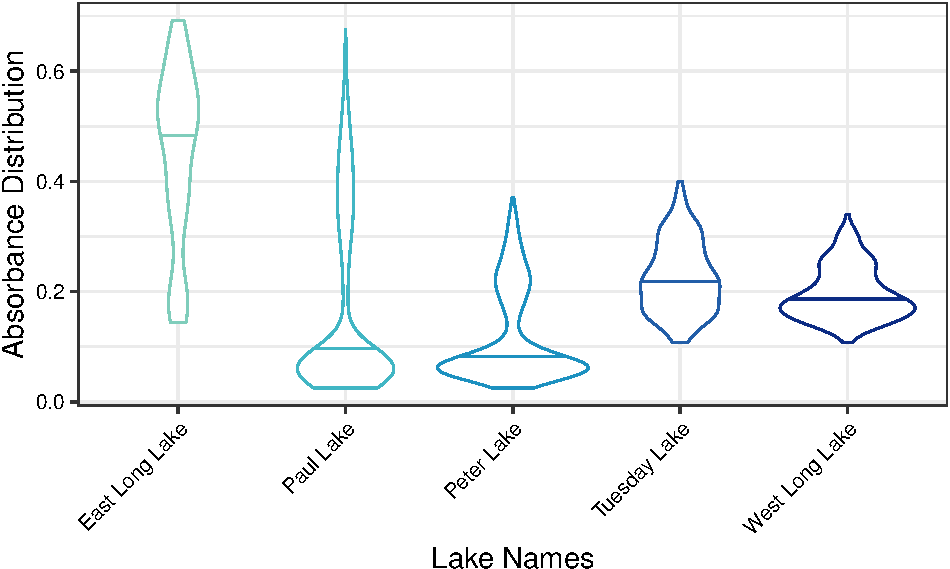
\includegraphics{Bash_ENV872_Project_files/figure-latex/vio-1.pdf}
\caption{\label{fig:vio}Absorbance differences by lake}
\end{figure}

\newpage

\subsection{Linear regression model}\label{linear-regression-model}

In order to determine what factors contribute to absorbance values, I
conducted a step-wise linear regression model. I was not able to include
DIC in the full model, because DIC was only measured at numeric depths
and not thermally stratified depths. Therefore, no data between
absorbance and DIC overlapped. The full model included the following
parameters: depth, DOC, Lake Name, and Total Particulate Carbon (TPC).

By performing a step-wise linear regression model, I can use the lowest
Akaike's Information Criterion (AIC) value to determine the ideal
statistical model that balances both simplicity and statistical power.
My regression analysis showed that all variables are significant and
allow us to best predict absorbance values. The resulting linear
expression is as follows:

\[Absorbance = 0.18(Epi*East) + 0.17(Hypo) + 0.02(DOC) -\]
\[0.18(Paul)  - 0.24(Peter) - 0.23(Tuesday) - 0.19(West) + 0.02(TPC) \]
For example, for every one unit increase in DOC, absorbance value
increases by 0.02 units. Alternatively, if absorbance is measured in
Peter Lake, absorbance will decrease by 0.24 units. The step function
shows that all variables, except for Metalimnion and PML depth
categories were significant predictors of absorbance, and the full model
had an adjusted R-squared value of 0.86, which is quite significant.
However, it is important to note that because of missing values within
each of the variables, there is an exceptionally high degrees of freedom
value of 1119.

\autoref{fig:lin} illustrates all predictors, with the exception of lake
name, and their relationship to absorbance.

\begin{Shaded}
\begin{Highlighting}[]
\CommentTok{#Step-wise linear regression}

\NormalTok{steplm <-}\StringTok{ }\KeywordTok{lm}\NormalTok{(}\DataTypeTok{data=}\NormalTok{carbon.data.processed, absorbance }\OperatorTok{~}\StringTok{ }\NormalTok{depth }\OperatorTok{+}\StringTok{ }\NormalTok{doc  }\OperatorTok{+}\StringTok{ }\NormalTok{lakename }\OperatorTok{+}\StringTok{ }\NormalTok{tpc)}
\KeywordTok{step}\NormalTok{(steplm) }
\end{Highlighting}
\end{Shaded}

\begin{verbatim}
## Start:  AIC=-6251.63
## absorbance ~ depth + doc + lakename + tpc
## 
##            Df Sum of Sq    RSS     AIC
## <none>                  4.3669 -6251.6
## - tpc       1    0.1978 4.5647 -6203.6
## - doc       1    0.5211 4.8880 -6126.4
## - lakename  4    3.2696 7.6365 -5628.7
## - depth     3    5.1414 9.5084 -5379.1
\end{verbatim}

\begin{verbatim}
## 
## Call:
## lm(formula = absorbance ~ depth + doc + lakename + tpc, data = carbon.data.processed)
## 
## Coefficients:
##            (Intercept)        depthHypolimnion        depthMetalimnion  
##               0.175600                0.171535                0.008826  
##               depthPML                     doc       lakenamePaul Lake  
##               0.005411                0.018642               -0.184280  
##     lakenamePeter Lake    lakenameTuesday Lake  lakenameWest Long Lake  
##              -0.241944               -0.229613               -0.188448  
##                    tpc  
##               0.018681
\end{verbatim}

\begin{Shaded}
\begin{Highlighting}[]
\CommentTok{#taking out none would result in the lowest AIC value}

\CommentTok{#full-model is the best, as shown by the step }
\NormalTok{fullmodel <-}\StringTok{ }\KeywordTok{lm}\NormalTok{(}\DataTypeTok{data=}\NormalTok{carbon.data.processed, absorbance }\OperatorTok{~}\StringTok{ }\NormalTok{depth }\OperatorTok{+}\StringTok{ }\NormalTok{doc  }\OperatorTok{+}\StringTok{ }\NormalTok{lakename }\OperatorTok{+}\StringTok{ }\NormalTok{tpc)}
\KeywordTok{summary}\NormalTok{(fullmodel)}
\end{Highlighting}
\end{Shaded}

\begin{verbatim}
## 
## Call:
## lm(formula = absorbance ~ depth + doc + lakename + tpc, data = carbon.data.processed)
## 
## Residuals:
##      Min       1Q   Median       3Q      Max 
## -0.27056 -0.03147 -0.00548  0.02536  0.38625 
## 
## Coefficients:
##                         Estimate Std. Error t value Pr(>|t|)    
## (Intercept)             0.175600   0.023113   7.598 6.35e-14 ***
## depthHypolimnion        0.171535   0.006031  28.441  < 2e-16 ***
## depthMetalimnion        0.008826   0.005946   1.484    0.138    
## depthPML                0.005411   0.006724   0.805    0.421    
## doc                     0.018642   0.001613  11.555  < 2e-16 ***
## lakenamePaul Lake      -0.184280   0.015929 -11.569  < 2e-16 ***
## lakenamePeter Lake     -0.241944   0.014605 -16.566  < 2e-16 ***
## lakenameTuesday Lake   -0.229613   0.009794 -23.444  < 2e-16 ***
## lakenameWest Long Lake -0.188448   0.011833 -15.926  < 2e-16 ***
## tpc                     0.018681   0.002624   7.119 1.94e-12 ***
## ---
## Signif. codes:  0 '***' 0.001 '**' 0.01 '*' 0.05 '.' 0.1 ' ' 1
## 
## Residual standard error: 0.06247 on 1119 degrees of freedom
##   (2294 observations deleted due to missingness)
## Multiple R-squared:  0.8584, Adjusted R-squared:  0.8572 
## F-statistic: 753.6 on 9 and 1119 DF,  p-value: < 2.2e-16
\end{verbatim}

\begin{figure}
\centering
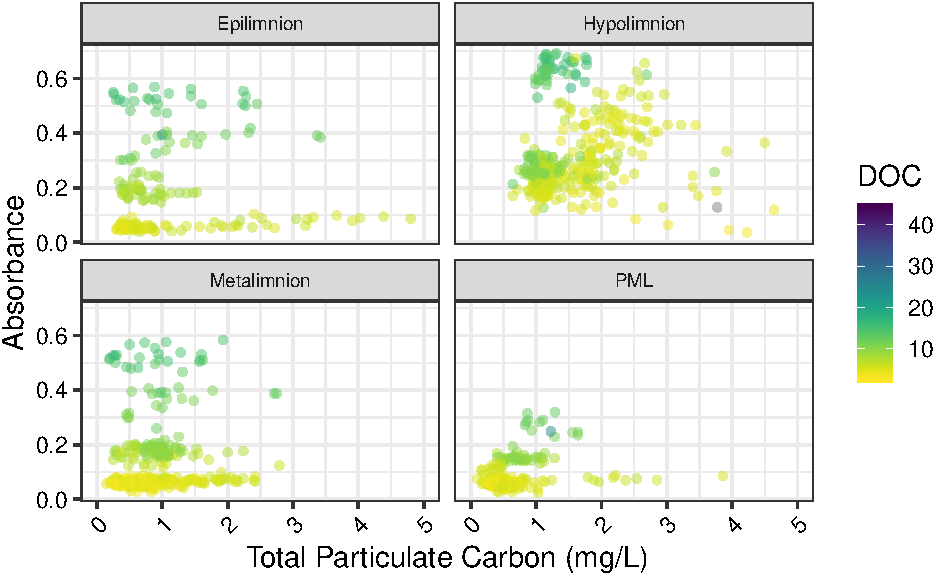
\includegraphics{Bash_ENV872_Project_files/figure-latex/lin-1.pdf}
\caption{\label{fig:lin}Facet plot of absorbance by TPC, DOC, and Depth}
\end{figure}

\newpage

\subsection{Time Series Analysis}\label{time-series-analysis}

A time series analysis will show whether absorbance values in lakes have
changed over time. I used a Mann Kendall test to determine whether there
is a monotonic overall trend in absorbance over time for the five lakes
of interest. While there is perhaps seasonality differences in
absorbance values, I am only interested in yearly trends, and so have
decided not to look at seasonal differences of absorbance.

To complete a time series analysis, I decided to split up the data by
lake so that I was able to determine whether there was a trend in each
lake. I also decided to filter the data by only observing absorbance
values at the Hypolimnion, which is the stratified column below the
thermocline at the bottom of the lake. I thought that choosing one depth
height would be appropriate, and I chose the bottom because I thought it
would be the most uniform layer among all lakes.

East Long Lake had a significant Mann Kendall test result, which
indicated a signicant negative monotonic trend over time (p-value =
2e-9). Using a series of pettitt tests and additional Mann Kendall
tests, I discovered three change points in East Long Lake's absorbance
data as well. West Long Lake also had significant negative trend from
the beginning to the end of the data, with one change point detected
(p-value = 1.18e-06). Peter and Tuesday Lakes both had a significant
over positive trend over time, meaning that the Mann Kendall test shows
that absorbance values in these lakes increased over time (p-value Peter
= 1.47e-06; p-value Tuesday= 0.0005). Both lakes also had two change
points. Lastly, Paul Lake's Mann Kendall test produced a non-significant
p-value, suggesting that there is no significant monotonic trend in
absorbance values over time (p-value = 0.10). However, a change point
was still detected in data.

\autoref{fig:time} summarizes and visualizes the findings.

\begin{Shaded}
\begin{Highlighting}[]
\CommentTok{#trimming data to only look at points of interest}
\NormalTok{carbon.data.processed.trimmed <-}\StringTok{ }\NormalTok{carbon.data.processed }\OperatorTok
\StringTok{  }\KeywordTok{filter}\NormalTok{(depth }\OperatorTok{==}\StringTok{ "Hypolimnion"}\NormalTok{) }\OperatorTok
\StringTok{  }\KeywordTok{select}\NormalTok{(absorbance, sampledate, lakename) }\OperatorTok
\StringTok{  }\KeywordTok{filter}\NormalTok{(sampledate }\OperatorTok{>}\StringTok{ }\KeywordTok{as.Date}\NormalTok{(}\StringTok{"1996-06-01"}\NormalTok{) }\OperatorTok{&}\StringTok{ }\NormalTok{sampledate }\OperatorTok{<}\StringTok{ }\KeywordTok{as.Date}\NormalTok{(}\StringTok{"2016-08-17"}\NormalTok{))}
\end{Highlighting}
\end{Shaded}

\subsubsection{East Long Lake}\label{east-long-lake}

\begin{Shaded}
\begin{Highlighting}[]
\CommentTok{#East Lake}
\NormalTok{East.mktest <-}\StringTok{ }\KeywordTok{filter}\NormalTok{(carbon.data.processed.trimmed, lakename }\OperatorTok{==}\StringTok{ "East Long Lake"}\NormalTok{)}

\CommentTok{#run MK test}
\KeywordTok{mk.test}\NormalTok{(East.mktest}\OperatorTok{$}\NormalTok{absorbance) }\CommentTok{#p=2e-9, so there is a significant negative trend from beginning to end of data}
\end{Highlighting}
\end{Shaded}

\begin{verbatim}
## 
##  Mann-Kendall trend test
## 
## data:  East.mktest$absorbance
## z = -5.9962, n = 73, p-value = 2.019e-09
## alternative hypothesis: true S is not equal to 0
## sample estimates:
##             S          varS           tau 
## -1260.0000000 44085.3333333    -0.4800003
\end{verbatim}

\begin{Shaded}
\begin{Highlighting}[]
\CommentTok{# Test for change point}
\KeywordTok{pettitt.test}\NormalTok{(East.mktest}\OperatorTok{$}\NormalTok{absorbance) }\CommentTok{#change point detected at place 30 1998-05-28}
\end{Highlighting}
\end{Shaded}

\begin{verbatim}
## 
##  Pettitt's test for single change-point detection
## 
## data:  East.mktest$absorbance
## U* = 1165, p-value = 2.151e-09
## alternative hypothesis: two.sided
## sample estimates:
## probable change point at time K 
##                              30
\end{verbatim}

\begin{Shaded}
\begin{Highlighting}[]
\CommentTok{#run second MK test for each change point range}
\KeywordTok{mk.test}\NormalTok{(East.mktest}\OperatorTok{$}\NormalTok{absorbance[}\DecValTok{1}\OperatorTok{:}\DecValTok{29}\NormalTok{]) }\CommentTok{#p=1e-5, significant positive trend in this range}
\end{Highlighting}
\end{Shaded}

\begin{verbatim}
## 
##  Mann-Kendall trend test
## 
## data:  East.mktest$absorbance[1:29]
## z = 4.4118, n = 29, p-value = 1.025e-05
## alternative hypothesis: true S is not equal to 0
## sample estimates:
##            S         varS          tau 
##  236.0000000 2837.3333333    0.5841656
\end{verbatim}

\begin{Shaded}
\begin{Highlighting}[]
\CommentTok{#test for change point}
\KeywordTok{pettitt.test}\NormalTok{(East.mktest}\OperatorTok{$}\NormalTok{absorbance[}\DecValTok{1}\OperatorTok{:}\DecValTok{29}\NormalTok{]) }\CommentTok{#change point detected at place 17 1997-06-12}
\end{Highlighting}
\end{Shaded}

\begin{verbatim}
## 
##  Pettitt's test for single change-point detection
## 
## data:  East.mktest$absorbance[1:29]
## U* = 185, p-value = 0.0005838
## alternative hypothesis: two.sided
## sample estimates:
## probable change point at time K 
##                              17
\end{verbatim}

\begin{Shaded}
\begin{Highlighting}[]
\KeywordTok{mk.test}\NormalTok{(East.mktest}\OperatorTok{$}\NormalTok{absorbance[}\DecValTok{1}\OperatorTok{:}\DecValTok{16}\NormalTok{]) }\CommentTok{#no trend}
\end{Highlighting}
\end{Shaded}

\begin{verbatim}
## 
##  Mann-Kendall trend test
## 
## data:  East.mktest$absorbance[1:16]
## z = 1.2156, n = 16, p-value = 0.2241
## alternative hypothesis: true S is not equal to 0
## sample estimates:
##           S        varS         tau 
##  28.0000000 493.3333333   0.2333333
\end{verbatim}

\begin{Shaded}
\begin{Highlighting}[]
\KeywordTok{mk.test}\NormalTok{(East.mktest}\OperatorTok{$}\NormalTok{absorbance[}\DecValTok{17}\OperatorTok{:}\DecValTok{29}\NormalTok{]) }\CommentTok{#no trend}
\end{Highlighting}
\end{Shaded}

\begin{verbatim}
## 
##  Mann-Kendall trend test
## 
## data:  East.mktest$absorbance[17:29]
## z = 1.5972, n = 13, p-value = 0.1102
## alternative hypothesis: true S is not equal to 0
## sample estimates:
##          S       varS        tau 
##  27.000000 265.000000   0.353009
\end{verbatim}

\begin{Shaded}
\begin{Highlighting}[]
\KeywordTok{mk.test}\NormalTok{(East.mktest}\OperatorTok{$}\NormalTok{absorbance[}\DecValTok{30}\OperatorTok{:}\DecValTok{73}\NormalTok{]) }\CommentTok{#significant negative trend over time}
\end{Highlighting}
\end{Shaded}

\begin{verbatim}
## 
##  Mann-Kendall trend test
## 
## data:  East.mktest$absorbance[30:73]
## z = -3.4795, n = 44, p-value = 0.0005024
## alternative hypothesis: true S is not equal to 0
## sample estimates:
##            S         varS          tau 
## -345.0000000 9774.3333333   -0.3648864
\end{verbatim}

\begin{Shaded}
\begin{Highlighting}[]
\KeywordTok{pettitt.test}\NormalTok{(East.mktest}\OperatorTok{$}\NormalTok{absorbance[}\DecValTok{30}\OperatorTok{:}\DecValTok{73}\NormalTok{]) }\CommentTok{#change point detected at place 17 (which means place 47 - 1999-06-09)}
\end{Highlighting}
\end{Shaded}

\begin{verbatim}
## 
##  Pettitt's test for single change-point detection
## 
## data:  East.mktest$absorbance[30:73]
## U* = 365, p-value = 0.0002071
## alternative hypothesis: two.sided
## sample estimates:
## probable change point at time K 
##                              17
\end{verbatim}

\begin{Shaded}
\begin{Highlighting}[]
\KeywordTok{mk.test}\NormalTok{(East.mktest}\OperatorTok{$}\NormalTok{absorbance[}\DecValTok{30}\OperatorTok{:}\DecValTok{46}\NormalTok{]) }\CommentTok{#no trend}
\end{Highlighting}
\end{Shaded}

\begin{verbatim}
## 
##  Mann-Kendall trend test
## 
## data:  East.mktest$absorbance[30:46]
## z = 0.82455, n = 17, p-value = 0.4096
## alternative hypothesis: true S is not equal to 0
## sample estimates:
##           S        varS         tau 
##  21.0000000 588.3333333   0.1549826
\end{verbatim}

\begin{Shaded}
\begin{Highlighting}[]
\KeywordTok{mk.test}\NormalTok{(East.mktest}\OperatorTok{$}\NormalTok{absorbance[}\DecValTok{47}\OperatorTok{:}\DecValTok{73}\NormalTok{]) }\CommentTok{#no trend}
\end{Highlighting}
\end{Shaded}

\begin{verbatim}
## 
##  Mann-Kendall trend test
## 
## data:  East.mktest$absorbance[47:73]
## z = 0, n = 27, p-value = 1
## alternative hypothesis: true S is not equal to 0
## sample estimates:
##             S          varS           tau 
## -1.000000e+00  2.301000e+03 -2.849003e-03
\end{verbatim}

\subsubsection{West Long Lake}\label{west-long-lake}

\begin{Shaded}
\begin{Highlighting}[]
\CommentTok{#split data by lake}
\NormalTok{West.mktest <-}\StringTok{ }\KeywordTok{filter}\NormalTok{(carbon.data.processed.trimmed, lakename }\OperatorTok{==}\StringTok{ "West Long Lake"}\NormalTok{)}

\CommentTok{#run MK test}
\KeywordTok{mk.test}\NormalTok{(West.mktest}\OperatorTok{$}\NormalTok{absorbance) }\CommentTok{#p is significant, so there is a significant negative trend from beginning to end of data}
\end{Highlighting}
\end{Shaded}

\begin{verbatim}
## 
##  Mann-Kendall trend test
## 
## data:  West.mktest$absorbance
## z = -4.8587, n = 87, p-value = 1.181e-06
## alternative hypothesis: true S is not equal to 0
## sample estimates:
##             S          varS           tau 
## -1326.0000000 74368.0000000    -0.3559285
\end{verbatim}

\begin{Shaded}
\begin{Highlighting}[]
\CommentTok{# Test for change point}
\KeywordTok{pettitt.test}\NormalTok{(West.mktest}\OperatorTok{$}\NormalTok{absorbance) }\CommentTok{#change point detected at place 44 1998-08-31}
\end{Highlighting}
\end{Shaded}

\begin{verbatim}
## 
##  Pettitt's test for single change-point detection
## 
## data:  West.mktest$absorbance
## U* = 1584, p-value = 3.057e-10
## alternative hypothesis: two.sided
## sample estimates:
## probable change point at time K 
##                              44
\end{verbatim}

\begin{Shaded}
\begin{Highlighting}[]
\CommentTok{#run second MK test for each change point range}
\KeywordTok{mk.test}\NormalTok{(West.mktest}\OperatorTok{$}\NormalTok{absorbance[}\DecValTok{1}\OperatorTok{:}\DecValTok{43}\NormalTok{]) }\CommentTok{#no trend}
\end{Highlighting}
\end{Shaded}

\begin{verbatim}
## 
##  Mann-Kendall trend test
## 
## data:  West.mktest$absorbance[1:43]
## z = 0.59704, n = 43, p-value = 0.5505
## alternative hypothesis: true S is not equal to 0
## sample estimates:
##            S         varS          tau 
## 5.800000e+01 9.114667e+03 6.469774e-02
\end{verbatim}

\begin{Shaded}
\begin{Highlighting}[]
\KeywordTok{mk.test}\NormalTok{(West.mktest}\OperatorTok{$}\NormalTok{absorbance[}\DecValTok{44}\OperatorTok{:}\DecValTok{87}\NormalTok{]) }\CommentTok{#no significant trend in this range}
\end{Highlighting}
\end{Shaded}

\begin{verbatim}
## 
##  Mann-Kendall trend test
## 
## data:  West.mktest$absorbance[44:87]
## z = 1.4676, n = 44, p-value = 0.1422
## alternative hypothesis: true S is not equal to 0
## sample estimates:
##            S         varS          tau 
##  146.0000000 9762.0000000    0.1553223
\end{verbatim}

\subsubsection{Peter Lake}\label{peter-lake}

\begin{Shaded}
\begin{Highlighting}[]
\CommentTok{#Peter Lake}
\NormalTok{Peter.mktest <-}\StringTok{ }\KeywordTok{filter}\NormalTok{(carbon.data.processed.trimmed, lakename }\OperatorTok{==}\StringTok{ "Peter Lake"}\NormalTok{) }\OperatorTok\StringTok{ }\KeywordTok{na.omit}\NormalTok{()}

\CommentTok{#run MK test}
\KeywordTok{mk.test}\NormalTok{(Peter.mktest}\OperatorTok{$}\NormalTok{absorbance) }\CommentTok{#p val is significant so there is a significant positive trend from beginning to end of data}
\end{Highlighting}
\end{Shaded}

\begin{verbatim}
## 
##  Mann-Kendall trend test
## 
## data:  Peter.mktest$absorbance
## z = 4.8159, n = 287, p-value = 1.465e-06
## alternative hypothesis: true S is not equal to 0
## sample estimates:
##            S         varS          tau 
## 7.826000e+03 2.640047e+06 1.911373e-01
\end{verbatim}

\begin{Shaded}
\begin{Highlighting}[]
\CommentTok{# Test for change point}
\KeywordTok{pettitt.test}\NormalTok{(Peter.mktest}\OperatorTok{$}\NormalTok{absorbance) }\CommentTok{#change point detected at place 202 2011-06-06}
\end{Highlighting}
\end{Shaded}

\begin{verbatim}
## 
##  Pettitt's test for single change-point detection
## 
## data:  Peter.mktest$absorbance
## U* = 7794, p-value = 4.25e-07
## alternative hypothesis: two.sided
## sample estimates:
## probable change point at time K 
##                             202
\end{verbatim}

\begin{Shaded}
\begin{Highlighting}[]
\CommentTok{#run second MK test for each change point range}
\KeywordTok{mk.test}\NormalTok{(Peter.mktest}\OperatorTok{$}\NormalTok{absorbance[}\DecValTok{1}\OperatorTok{:}\DecValTok{201}\NormalTok{]) }\CommentTok{#p>0.05, no significant trend in this date range}
\end{Highlighting}
\end{Shaded}

\begin{verbatim}
## 
##  Mann-Kendall trend test
## 
## data:  Peter.mktest$absorbance[1:201]
## z = -0.89267, n = 201, p-value = 0.372
## alternative hypothesis: true S is not equal to 0
## sample estimates:
##             S          varS           tau 
## -8.520000e+02  9.088247e+05 -4.250453e-02
\end{verbatim}

\begin{Shaded}
\begin{Highlighting}[]
\KeywordTok{mk.test}\NormalTok{(Peter.mktest}\OperatorTok{$}\NormalTok{absorbance[}\DecValTok{202}\OperatorTok{:}\DecValTok{287}\NormalTok{]) }\CommentTok{#significant positive trend over time}
\end{Highlighting}
\end{Shaded}

\begin{verbatim}
## 
##  Mann-Kendall trend test
## 
## data:  Peter.mktest$absorbance[202:287]
## z = 4.0658, n = 86, p-value = 4.786e-05
## alternative hypothesis: true S is not equal to 0
## sample estimates:
##            S         varS          tau 
## 1.091000e+03 7.187167e+04 2.989044e-01
\end{verbatim}

\begin{Shaded}
\begin{Highlighting}[]
\KeywordTok{pettitt.test}\NormalTok{(Peter.mktest}\OperatorTok{$}\NormalTok{absorbance[}\DecValTok{202}\OperatorTok{:}\DecValTok{287}\NormalTok{]) }\CommentTok{#change point detected at place 50 (which means place 50+202=252 - 2014-06-30)}
\end{Highlighting}
\end{Shaded}

\begin{verbatim}
## 
##  Pettitt's test for single change-point detection
## 
## data:  Peter.mktest$absorbance[202:287]
## U* = 1301, p-value = 2.796e-07
## alternative hypothesis: two.sided
## sample estimates:
## probable change point at time K 
##                              50
\end{verbatim}

\begin{Shaded}
\begin{Highlighting}[]
\KeywordTok{mk.test}\NormalTok{(Peter.mktest}\OperatorTok{$}\NormalTok{absorbance[}\DecValTok{202}\OperatorTok{:}\DecValTok{251}\NormalTok{]) }\CommentTok{#no trend}
\end{Highlighting}
\end{Shaded}

\begin{verbatim}
## 
##  Mann-Kendall trend test
## 
## data:  Peter.mktest$absorbance[202:251]
## z = -1.9409, n = 50, p-value = 0.05227
## alternative hypothesis: true S is not equal to 0
## sample estimates:
##             S          varS           tau 
##  -233.0000000 14287.6666667    -0.1905154
\end{verbatim}

\begin{Shaded}
\begin{Highlighting}[]
\KeywordTok{mk.test}\NormalTok{(Peter.mktest}\OperatorTok{$}\NormalTok{absorbance[}\DecValTok{252}\OperatorTok{:}\DecValTok{287}\NormalTok{]) }\CommentTok{#no trend}
\end{Highlighting}
\end{Shaded}

\begin{verbatim}
## 
##  Mann-Kendall trend test
## 
## data:  Peter.mktest$absorbance[252:287]
## z = 0.29974, n = 36, p-value = 0.7644
## alternative hypothesis: true S is not equal to 0
## sample estimates:
##            S         varS          tau 
## 2.300000e+01 5.387000e+03 3.659517e-02
\end{verbatim}

\subsubsection{Paul Lake}\label{paul-lake}

\begin{Shaded}
\begin{Highlighting}[]
\CommentTok{#Paul Lake}
\NormalTok{Paul.mktest <-}\StringTok{ }\KeywordTok{filter}\NormalTok{(carbon.data.processed.trimmed, lakename }\OperatorTok{==}\StringTok{ "Paul Lake"}\NormalTok{) }\OperatorTok\StringTok{ }\KeywordTok{na.omit}\NormalTok{()}

\CommentTok{#run MK test}
\KeywordTok{mk.test}\NormalTok{(Paul.mktest}\OperatorTok{$}\NormalTok{absorbance) }\CommentTok{#p>0.05 so no significant over time}
\end{Highlighting}
\end{Shaded}

\begin{verbatim}
## 
##  Mann-Kendall trend test
## 
## data:  Paul.mktest$absorbance
## z = -1.6421, n = 291, p-value = 0.1006
## alternative hypothesis: true S is not equal to 0
## sample estimates:
##             S          varS           tau 
## -2.725000e+03  2.751921e+06 -6.466546e-02
\end{verbatim}

\begin{Shaded}
\begin{Highlighting}[]
\CommentTok{# Test for change point}
\KeywordTok{pettitt.test}\NormalTok{(Paul.mktest}\OperatorTok{$}\NormalTok{absorbance) }\CommentTok{#change point detected at place 72 2001-08-20}
\end{Highlighting}
\end{Shaded}

\begin{verbatim}
## 
##  Pettitt's test for single change-point detection
## 
## data:  Paul.mktest$absorbance
## U* = 4575, p-value = 0.01245
## alternative hypothesis: two.sided
## sample estimates:
## probable change point at time K 
##                              72
\end{verbatim}

\begin{Shaded}
\begin{Highlighting}[]
\CommentTok{#run second MK test for each change point range}
\KeywordTok{mk.test}\NormalTok{(Paul.mktest}\OperatorTok{$}\NormalTok{absorbance[}\DecValTok{1}\OperatorTok{:}\DecValTok{71}\NormalTok{]) }\CommentTok{#no trend}
\end{Highlighting}
\end{Shaded}

\begin{verbatim}
## 
##  Mann-Kendall trend test
## 
## data:  Paul.mktest$absorbance[1:71]
## z = -1.1566, n = 71, p-value = 0.2474
## alternative hypothesis: true S is not equal to 0
## sample estimates:
##             S          varS           tau 
## -2.340000e+02  4.058333e+04 -9.425987e-02
\end{verbatim}

\begin{Shaded}
\begin{Highlighting}[]
\KeywordTok{mk.test}\NormalTok{(Paul.mktest}\OperatorTok{$}\NormalTok{absorbance[}\DecValTok{72}\OperatorTok{:}\DecValTok{291}\NormalTok{]) }\CommentTok{#no trend}
\end{Highlighting}
\end{Shaded}

\begin{verbatim}
## 
##  Mann-Kendall trend test
## 
## data:  Paul.mktest$absorbance[72:291]
## z = 1.7089, n = 220, p-value = 0.08747
## alternative hypothesis: true S is not equal to 0
## sample estimates:
##            S         varS          tau 
## 1.866000e+03 1.191044e+06 7.756263e-02
\end{verbatim}

\subsubsection{Tuesday Lake}\label{tuesday-lake}

\begin{Shaded}
\begin{Highlighting}[]
\CommentTok{#Tuesday}
\NormalTok{Tuesday.mktest <-}\StringTok{ }\KeywordTok{filter}\NormalTok{(carbon.data.processed.trimmed, lakename }\OperatorTok{==}\StringTok{ "Tuesday Lake"}\NormalTok{) }\OperatorTok\StringTok{ }\KeywordTok{na.omit}\NormalTok{()}

\CommentTok{#run MK test}
\KeywordTok{mk.test}\NormalTok{(Tuesday.mktest}\OperatorTok{$}\NormalTok{absorbance) }\CommentTok{#p is significant, so there is a significant positive trend from beginning to end of data}
\end{Highlighting}
\end{Shaded}

\begin{verbatim}
## 
##  Mann-Kendall trend test
## 
## data:  Tuesday.mktest$absorbance
## z = 3.4932, n = 102, p-value = 0.0004773
## alternative hypothesis: true S is not equal to 0
## sample estimates:
##            S         varS          tau 
## 1.209000e+03 1.195877e+05 2.353522e-01
\end{verbatim}

\begin{Shaded}
\begin{Highlighting}[]
\CommentTok{# Test for change point}
\KeywordTok{pettitt.test}\NormalTok{(Tuesday.mktest}\OperatorTok{$}\NormalTok{absorbance) }\CommentTok{#change point detected at place 68 2014-06-25}
\end{Highlighting}
\end{Shaded}

\begin{verbatim}
## 
##  Pettitt's test for single change-point detection
## 
## data:  Tuesday.mktest$absorbance
## U* = 1824, p-value = 1.626e-08
## alternative hypothesis: two.sided
## sample estimates:
## probable change point at time K 
##                              68
\end{verbatim}

\begin{Shaded}
\begin{Highlighting}[]
\CommentTok{#run second MK test for each change point range}
\KeywordTok{mk.test}\NormalTok{(Tuesday.mktest}\OperatorTok{$}\NormalTok{absorbance[}\DecValTok{1}\OperatorTok{:}\DecValTok{67}\NormalTok{]) }\CommentTok{#p<0.05, significant negative trend in this range}
\end{Highlighting}
\end{Shaded}

\begin{verbatim}
## 
##  Mann-Kendall trend test
## 
## data:  Tuesday.mktest$absorbance[1:67]
## z = -3.3124, n = 67, p-value = 0.0009249
## alternative hypothesis: true S is not equal to 0
## sample estimates:
##             S          varS           tau 
##  -613.0000000 34135.6666667    -0.2780056
\end{verbatim}

\begin{Shaded}
\begin{Highlighting}[]
\CommentTok{#test for change point}
\KeywordTok{pettitt.test}\NormalTok{(Tuesday.mktest}\OperatorTok{$}\NormalTok{absorbance[}\DecValTok{1}\OperatorTok{:}\DecValTok{67}\NormalTok{]) }\CommentTok{#change point detected at place 44 2012-08-22}
\end{Highlighting}
\end{Shaded}

\begin{verbatim}
## 
##  Pettitt's test for single change-point detection
## 
## data:  Tuesday.mktest$absorbance[1:67]
## U* = 712, p-value = 9.409e-05
## alternative hypothesis: two.sided
## sample estimates:
## probable change point at time K 
##                              44
\end{verbatim}

\begin{Shaded}
\begin{Highlighting}[]
\KeywordTok{mk.test}\NormalTok{(Tuesday.mktest}\OperatorTok{$}\NormalTok{absorbance[}\DecValTok{1}\OperatorTok{:}\DecValTok{43}\NormalTok{]) }\CommentTok{#no trend}
\end{Highlighting}
\end{Shaded}

\begin{verbatim}
## 
##  Mann-Kendall trend test
## 
## data:  Tuesday.mktest$absorbance[1:43]
## z = 0.8898, n = 43, p-value = 0.3736
## alternative hypothesis: true S is not equal to 0
## sample estimates:
##            S         varS          tau 
## 8.600000e+01 9.125333e+03 9.550287e-02
\end{verbatim}

\begin{Shaded}
\begin{Highlighting}[]
\KeywordTok{mk.test}\NormalTok{(Tuesday.mktest}\OperatorTok{$}\NormalTok{absorbance[}\DecValTok{44}\OperatorTok{:}\DecValTok{67}\NormalTok{]) }\CommentTok{#no trend}
\end{Highlighting}
\end{Shaded}

\begin{verbatim}
## 
##  Mann-Kendall trend test
## 
## data:  Tuesday.mktest$absorbance[44:67]
## z = -0.62049, n = 24, p-value = 0.5349
## alternative hypothesis: true S is not equal to 0
## sample estimates:
##             S          varS           tau 
##  -26.00000000 1623.33333333   -0.09454608
\end{verbatim}

\begin{Shaded}
\begin{Highlighting}[]
\KeywordTok{mk.test}\NormalTok{(Tuesday.mktest}\OperatorTok{$}\NormalTok{absorbance[}\DecValTok{68}\OperatorTok{:}\DecValTok{102}\NormalTok{]) }\CommentTok{#no trend}
\end{Highlighting}
\end{Shaded}

\begin{verbatim}
## 
##  Mann-Kendall trend test
## 
## data:  Tuesday.mktest$absorbance[68:102]
## z = 0.53976, n = 35, p-value = 0.5894
## alternative hypothesis: true S is not equal to 0
## sample estimates:
##            S         varS          tau 
## 3.900000e+01 4.956333e+03 6.565666e-02
\end{verbatim}

\begin{figure}
\centering
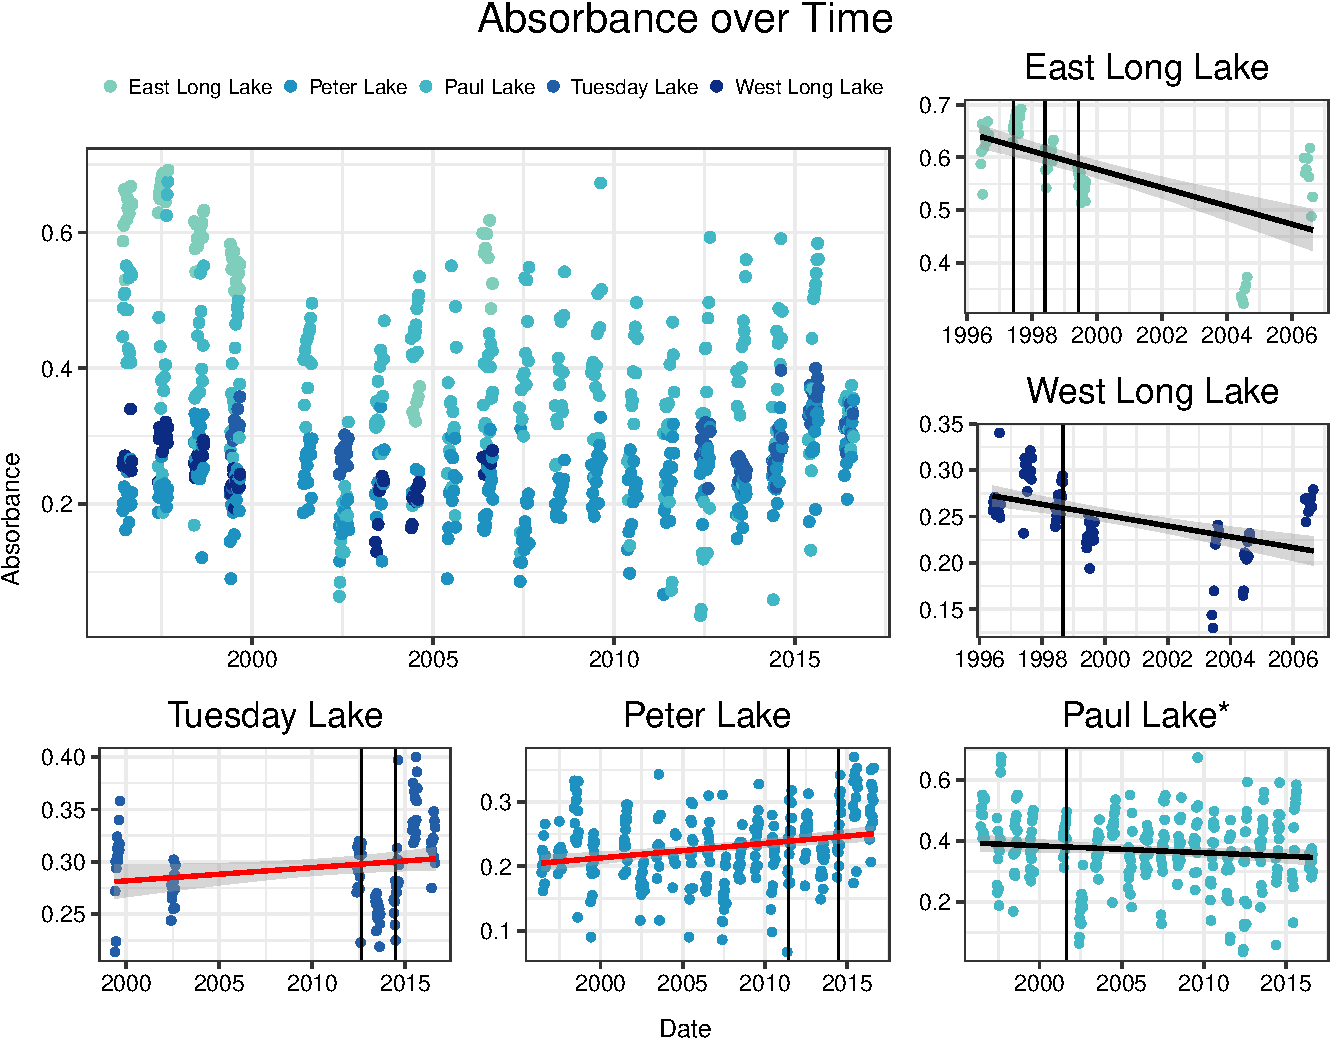
\includegraphics{Bash_ENV872_Project_files/figure-latex/time-1.pdf}
\caption{\label{fig:time} Absorbance in East Long Lake, West Long Lake,
Peter Lake, Paul Lake, and Tuesday Lake over time}
\end{figure}

\begin{verbatim}
## TableGrob (5 x 4) "arrange": 9 grobs
##   z     cells    name                grob
## 1 1 (2-3,2-3) arrange      gtable[layout]
## 2 2 (2-2,4-4) arrange      gtable[layout]
## 3 3 (3-3,4-4) arrange      gtable[layout]
## 4 4 (4-4,2-2) arrange      gtable[layout]
## 5 5 (4-4,3-3) arrange      gtable[layout]
## 6 6 (4-4,4-4) arrange      gtable[layout]
## 7 7 (1-1,2-4) arrange text[GRID.text.799]
## 8 8 (5-5,2-4) arrange text[GRID.text.800]
## 9 9 (1-5,1-1) arrange text[GRID.text.801]
\end{verbatim}

\newpage

\section{Summary and Conclusions}\label{summary-and-conclusions}

Absorbance is able to be predicted by lake, depth, total particulate
carbon, and dissolved organic carbon concentration. The model that
included all of these variables were able to explain 85\% of the
variation of absorbance within the data. Absorbance values are also
significantly different in all five lakes examined, as determined by the
Kruskal Wallis and Dunn Tests.

It is important to note that while these results are desirable and seem
to explain a lot of the variation, there are many other factors that can
contribute to absorbance values that were not measured in this dataset.
Color of the lake, total depth of the lake, phytoplankton and its
pigments, organic materials that were filtered out, and many other
potential contributors were not considered. While depth was a variable,
only the depth category of Hypolimnion was considered, which did not
take into account the total depth of the water in the lake. Absorbance
can also be measured at different wavelengths to determine the peak
absorbance curve for different substances. The absorption of light also
affects the amount of total energy captured by a substance.

Absorbance characteristics of lakes can inform researchers of valuable
information about other characteristics of the lakes that may not be
measureable (Beaucler, 2001). Because absorbance is relatively easy to
measure with a spectrophotometer, absorbance spectroscopy can be used to
characterize and predict other characteristics. It can be an indication
of the aesthetic quality of lakes, amount of DOC or algae or other
substances in lakes, retention time, or even latitude (Erlandsson et
al., 2012).

Absorption of light in lakes is a great phenomenon that is easy to study
and gives information about many other aspects of the lake's ecosystem.
Understanding the relationship between absorbance, depth of the water,
DOC content, and TPC content gives us a clearer understanding of the
biology and physical characteristics of the five examined lakes in this
larger dataset from the Northern Temperate Lakes project.

\newpage

\section{References}\label{references}

Beaucler, K. B., \& Gunn, J. M. (2001). Ultraviolet absorbance in lakes
near the metal smelters in Sudbury, Canada. Journal of Environmental
Monitoring: JEM, 3(6), 575--579.

Erlandsson, Martin \& Futter, Martyn \& Kothawala, D \& Köhler, S.
(2012). Variability in spectral absorbance metrics across boreal lake
waters. Journal of environmental monitoring : JEM. 14. 2643-52.
10.1039/c2em30266g.

Thrane, JE., Hessen, D.O. \& Andersen, T. Ecosystems (2014) 17: 1040.
\url{https://doi.org/10.1007/s10021-014-9776-2}


\end{document}
